\documentclass{lxaiproposal}


%   \usepackage[english,french]{babel}   % "babel.sty" + "french.sty"
\usepackage[english]{babel}   % "babel.sty" + "french.sty"

% \usepackage[english,francais]{babel} % "babel.sty"
% \usepackage{french}                  % "french.sty"
\usepackage{times}            % ajout times le 30 mai 2003

\usepackage{epsfig}
\usepackage{graphicx}
\usepackage{amsmath}
\usepackage{amssymb}
\usepackage{booktabs}
\usepackage{multirow}
\usepackage{pifont}
\usepackage{caption}
\usepackage{subcaption}

\usepackage{amsmath}
\usepackage{mathtools}
\usepackage{amssymb}
\usepackage{algorithm}
\usepackage[noend]{algpseudocode}


\usepackage{array}
\usepackage{color}
\usepackage{colortbl}

\usepackage{pifont}
\usepackage{amssymb}
\usepackage{latexsym}

\usepackage{booktabs}

%% --------------------------------------------------------------
%% FONTS CODING ?
% \usepackage[OT1]{fontenc} % Old fonts
% \usepackage[T1]{fontenc}  % New fonts (preferred)
%% ==============================================================

\title{ECSE 6810 Final Project \\ DAG Structure Learning using Generative Flow Networks}

\author{\coord{Ali}{Najibi}{}\\\\
\coord{\textbf{Course Instructor: Prof. Qiang}}{\textbf{Ji}}{}
}

\address{\affil{}{Rensselaer Polytechnic Institute}
}

%% If all authors have the same address %%%%%%%%%%%%%%%%%%%%%%%%%%%%%%%%%%%%%%%
%                                                                             %
%   \auteur{\coord{Michel}{Dupont}{},                                         %
%           \coord{Marcel}{Dupond}{},                                         %
%           \coord{Michelle}{Durand}{},                                       %
%           \coord{Marcelle}{Durand}{}}                                       %
%                                                                             %
%   \adress{\affil{}{Laboratoire Traitement des Signaux et des Images \\      %
%     1 rue de la Science, BP 00000, 99999 Nouvelleville Cedex 00, France}}   %
%                                                                             %
%                                                                             %
%%%%%%%%%%%%%%%%%%%%%%%%%%%%%%%%%%%%%%%%%%%%%%%%%%%%%%%%%%%%%%%%%%%%%%%%%%%%%%%

\email{}

\englishabstract{
    Directed Acyclic Graphs (DAGs) are widely used in modeling complex systems where relationships are directional
    and non-cyclic. Using these graphs, we can model complex distributions and perform inference tasks. There are
    multiple algorithms to learn the structure of a DAG from data including ......}

\begin{document}
    \maketitle
%


    \section{Introduction}
    \vspace*{-3mm}

    Bayesian Networks (BNs) are powerful tools for modeling complex systems where relationships are directional and
    non-cyclic. A BN consists of a DAG $G$ where each node represents a random variable and edges
    represent the conditional dependencies between the variables. Moreover, each BN has a set of parameters $\theta$ that
    represent the conditional probability distributions of each variable given its parents.

    The Major characteristic of BNs that make them extremely useful in modeling probability distributions is the
    conditional independence property. This property states that a variable $X$ is conditionally independent of its
    non-descendants given its parents. This property allows us to factorize the joint probability distribution of the
    variables in the graph as follows:
    \begin{equation}
        P(X_1, X_2, \ldots, X_n) = \prod_{i=1}^{n} P(X_i | \text{Pa}(X_i))
        \label{eq:bn_factorization}
    \end{equation}
    where $\text{Pa}(X_i)$ denotes the parents of variable $X_i$ in the graph.

    Learning a target distribution $P(X)$ from data $D$ is a fundamental problem in machine learning. In the context of
    BNs, this problem is to learn the structure of the DAG $G$ and the parameters $\theta$ that best represent the
    distribution $P(X|D)$. To achieve that, we can factorize $P(X|D)$ as:
    \begin{equation}
        P(X|D) = \sum_{G} P(G|D) P(\theta|G,D) P(X|G,\theta,D)
        \label{eq:bn_learning}
    \end{equation}
    where $P(G|D)$ is the posterior distribution of the DAG given the data, $P(\theta|G,D)$ is the posterior distribution
    of the parameters given the DAG and the data, and $P(X|G,\theta,D)$ is the likelihood of the data given the DAG and
    the parameters.


    A central problem in Bayesian Networks is structure learning — identifying the DAG $G$ and parameters
    $\theta$ that best explain the observed data $D$. This process typically involves approximating the posterior
    distribution $P(G\mid D)$, a computationally intensive task due to the combinatorial nature of
    possible DAGs. Conventional methods like Markov Chain Monte Carlo (MCMC) and Variational Inference address this
    challenge but often face limitations such as slow convergence and computational inefficiencies.

    Generative Flow Networks (GFlowNets)~\cite{bengio2023gflownetfoundations}, recently introduced as a novel
    probabilistic modeling paradigm, can be leveraged to model this distribution as a sequential decision-making
    problem. By treating DAG construction as a sequential decision-making problem, GFlowNets approximate the
    posterior $P(G\mid D)$ by sampling DAGs through learned transition probabilities. This approach provides notable
    advantages over traditional methods, including improved scalability and guaranteed adherence to acyclicity
    constraints. To this end, we w

    In this project, we want to explore the potential of GFlowNets in learning the structure of a DAG from data. We
    will implement the proposed approach in the original paper~\cite{deleu2022daggflownet} and evaluate its performance
    on synthetic data. We will compare the results using various evaluation metrics including SHD, E-SHD, Ancestor
    Relationship, and BGe score.
    .......

    The following sections of this report are organized as follows. In Section~\ref{sec:related_work}, we provide a
    brief overview of the related work including the main algorithms used in for learning $\P(G|D)$. Then, we proceed
    to describe the main concepts and algorithms used in this project in Section~\ref{sec:background}. In Section~\ref{sec:proposed_approach},
    we describe the proposed approach for learning the structure of a DAG using generative flow networks in the
    original paper~\cite{deleu2022daggflownet}. Later we will describe and comprehensively explain the experiments
    conducted in this project in Section~\ref{sec:experiments}. Section~\ref{sec:results} will present the results of the
    experiments and discuss the findings. Finally, we will conclude the report in Section~\ref{sec:conclusion}
    followed by Section~\ref{sec:future_work} where we will discuss the future work.


    \section{Related Work}\label{sec:related_work}
    \vspace*{-3mm}

    In this section, we provide a brief overview of the main algorithms used for learning the structure of a DAG from
    data.

    \subsection{Markov Chain Monte Carlo (MCMC)}
    \vspace*{-3mm}
    The process of learning a posterior distribution $P(G|D)$ is computationally intensive; thus, the first idea that
    comes to mind is to sample from this distribution instead of completely learning it. Markov Chain Monte Carlo (MCMC)
    is the most effective and widely used method for sampling method. MCMC methods are based on the idea of constructing
    a Markov chain that has the desired distribution as its stationary distribution. Multiple approaches \cite{
        mcmc1, mcmc2, mcmc3} have been proposed to sample from the posterior distribution of the DAG given the data.
    However, these methods are computationally expensive and often face limitations such as slow convergence and
    computational inefficiencies. Recently in~\cite{viinikka2020scalablebayesianlearningcausal}, Viinikka et al. proposed a scalable approach towards
    learning the structure of a DAG using MCMC methods.

    \subsection{Variational Inference}
    \vspace*{-3mm}

    Variational Inference (VI) is another popular method for approximating the posterior distribution $P(G|D)$. VI
    methods are based on the idea of approximating the posterior distribution with a simpler distribution that is easier
    to sample from. Methods leveraging this approach mostly use Gradient-based methods to minimize the difference
    between the true posterior and the approximated posterior. In~\cite{cundy2021bcdnetsscalablevariational}, Cundy et al. proposed a scalable
    approach for learning the structure of a DAG using Variational Inference; they tried to address the limitation
    decomposing the adjacency matrix into a triangular matrix and a permutation. Other methods like~\cite{annadani2021variationalcausalnetworksapproximate, lorch2021dibsdifferentiablebayesianstructure}
    try to relax the acyclicity constraint into a soft prior $P(G)$ considering continuous acyclicity.


    \section{Background}\label{sec:background}
    \vspace*{-3mm}

    The problem of learning the structure of a DAG from data could be formulated as learning the transition probabilities
    of a Markov Chain where each state represents a DAG. In such a formulation, the goal is to learn these
    transition probabilities such that the probability of seeing each state is proportional to the posterior probability
    of the DAG given the data. This process could be modeled as a sequential decision-making problem.
    DAG-GFlowNet~\cite{deleu2022daggflownet} is a novel approach that leverages Generative Flow Networks (GFlowNets) to
    model $P(G|\mid D)$.

    \subsection{Generative Flow Networks}
    \vspace*{-3mm}

    Suppose we have a sampling space $\mathcal{X}$ and a target distribution $P(X)$. The goal of Generative Flow
    Networks (GFlowNets) is to model this distribution by generating samples $X \in \mathcal{X}$ with probabilities
    proportional to a given reward function $R(X)$, such that $P(X) \propto R(X)$. To achieve this, GFlowNets treat
    the generation of samples as a sequential decision-making process over a Directed Acyclic Graph (DAG) of states.

    GFlowNet has an internal DAG of states $s \in \mathcal{S}$, where each state represents a partial or complete
    sample, starting from an initial state $s_0$ and terminating at a special absorbing state $s_f$. Note that only
    complete states are connected to the absorbing state.

    Transitions between states are guided by learned
    probabilities, and the task is to ensure that the flow of probabilities through the states satisfies the
    \textit{flow-matching condition}~\eqref{eq:flow_matching} at each state $s \in \mathcal{S}$. This condition
    ensures that the total incoming flow to a state equals the outgoing flow plus the reward at that state.

    \begin{equation}
        \sum_{s \in \text{Pa}(s')} F(s \to s') = \sum_{s'' \in \text{Ch}(s')} F(s' \to s'') + R(s'),
        \label{eq:flow_matching}
    \end{equation}

    where $F(s \to s')$ is the flow between states $s$ and $s'$, and $\text{Pa}(s')$ and $\text{Ch}(s')$ are the
    parent and child states of $s'$, respectively. Note that the $R(s) = 0$ for any incomplete state
    $s \in \mathcal{S}\setminus\mathcal{X}$ and is positive for complete states $s \in \mathcal{X}$.

    If the flow-matching condition~\eqref{eq:flow_matching} is satisfied, GFlowNet induces a generative process to
    sample complete states $s \in \mathcal{X}$ with probability proportional to the reward function $R(s)$. In other
    words, starting from the initial state $s_0$, the generative process will traverse the DAG of states, sampling
    each state $s_i$ using the transition probabilities defined as normalized outgoing flows consistent with~
    \eqref{eq:flow_prob}.

    \begin{equation}
        P(s_{i+1} \mid s_i) \propto F(s_i \to s_{i+1}),
        \label{eq:flow_prob}
    \end{equation}

    This process, will result in a sample $s$ with probability $P(s) \propto R(s)$. In other words, consider~
    \eqref{eq:flow_matching} equation, there are two explanations for a high reward $R(s)$: either the flow from the parent
    states is high or the flow to the child states is low. This is the key idea behind GFlowNets.


    \textbf{Detailed-Balance Condition} One challenge that exists in formulating the flow-matching condition is that it
    tends to be orders of magnitude larger as we get closer to the intial state --- this is due to the fact that the
    initial state scaters the whole flow of the network and thus, contains $\sum_{s \in \mathcal{X}} R(s)$ flow.

    Such difference in flow values makes it difficult to parametrize $F$. Authors used proposed alternative by Bengio
    et al. in~\cite{bengio2023gflownetfoundations} to address this issue. This approach suggests parametrization of
    forward and backward transition probabilities $P_{\phi}(s_{i+1} \mid s_i)$ and $P_{\psi}(s_i \mid s_{i+1})$ such
    that the flow-matching condition is satisfied through eq.~\eqref{eq:detailed_balance}.

    This equation --- proof could be seen in Appendix~\ref{app:detailed_balance} --- holds in the case that all states of the GFlowNet are
    complete (except the terminal state $s_f$). Moreover, $P_{\phi}(s_{i+1} \mid s_i)$ is an encoding of the forward
    flow --- a distribution over the child states of $s_i$ --- and $P_{\psi}$ is an encoding of the backward flow --- a
    distribution over the parent states of $s_{i+1}$. Eq.~\eqref{eq:detailed_balance} ensures that the flow-matching
    condition holds for any transition $s_i \to s_{i+1}$.

    \begin{equation}
        \begin{aligned}
            R(s_i) P_{\phi}(s_{i+1} \mid s_i)P_{\phi}(s_f \mid s_{i+1})=\\
            R(s_{i+1}) P_{\psi}(s_i \mid s_{i+1})P_{\phi}(s_f \mid s_i)
        \end{aligned}
        \label{eq:detailed_balance}
    \end{equation}


    \section{Proposed Approach}\label{sec:proposed_approach}

    \subsection{GFlowNet for DAG Structure Learning}

    The proposed approach in~\cite{deleu2022daggflownet} leverages Generative Flow Networks (GFlowNets) to model the
    posterior distribution $P(G|D)$ of a DAG given data $D$. The goal is to learn the transition probabilities of a
    Markov Chain where each state represents a valid DAG$G$.

    To further elaborate this notion, first, let's take a look at Fig.~\ref{fig:dag_gflownet}. This figure shows the
    overall generation process of a DAG using GFlowNet. The process starts from an initial state $G_0$ and moves
    forward, according to the transition probabilities, $P_{\phi}(G_{i+1} \mid G_i)$ until it reaches the absorbing state
    $s_f$. Note that since in eq.~\eqref{eq:detailed_balance} we assumed that all states are complete except the
    absorbing state, all states of the inner DAG of GFlowNet should be valid DAGs (except the absorbing state).
    At each step, moving from $G_i$ to $G_{i+1}$, we add an edge to the DAG considering the acyclicity constraint.
    The aciclicity constraint is enforced using some masking operation on the adjacency matrix of the DAG which is
    explained in details in Appendix~\ref{app:masking}.


    \begin{figure}[h]
        \centering
        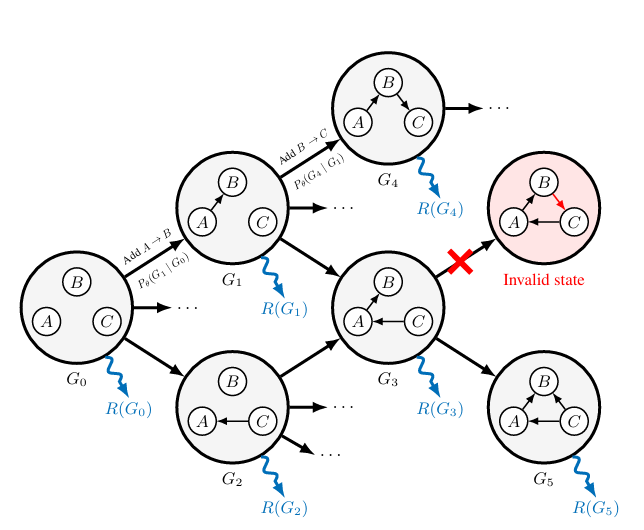
\includegraphics[width=0.5\textwidth]{figures/dag_gflownet}
        \caption{DAG-GFlowNet: Generative Flow Network for DAG Structure Learning for 3 nodes. Figure taken from~\cite{deleu2022daggflownet}.}
        \label{fig:dag_gflownet}
    \end{figure}

    To parameterize the forward transition probabilities $P_{\phi}(G_{i+1} \mid G_i)$, the authors have distinguished
    between two types of transition, terminating transition $P_{\phi}(s_f \mid G_i)$ and non-terminating transition
    $P_{\phi}(G_{i+1} \mid G_i)$.
    More accurately, the non-terminating transition should be written as:
    \begin{equation}
        P_{\phi}(G_{i+1} \mid G_i) = (1-P_{\phi}(s_f \mid G_i)) P_{\phi}(G_{i+1} \mid G_i, \neg s_f)
        \label{eq:non_terminating_transition}
    \end{equation}
    where $P_{\phi}(G_{i+1} \mid G_i, \neg s_f)$ is the transition probability from $G_i$ to $G_{i+1}$ knowing we do not
    terminate.

    Simply put, $G_{i+1}$ is the result of adding an edge to $G_i$, thus, $P_{\phi}(G_{i+1} \mid G_i, \neg s_f)$ can
    be modeled
    as a probability distribution over all the possible moves $d^2$ --- where $d$ is the number of nodes in the graph ---
    that can be made to $G_i$ to get $G_{i+1}$. However, to account for the acyclicity constraint, the authors have
    proposed filtering out actions not leading to valid DAGs and setting their probabilities to zero. Then, normalizing
    the remaining probabilities to sum to one.

    \subsection{Neural Network Architecture}\label{sec:nn_architecture}
    \vspace*{-3mm}

    Eq.~\eqref{eq:non_terminating_transition} suggests that the transition probabilities could be modeled using the
    same backbone with $\phi$ as the parameters and different heads in the output layer. The authors used a neural
    network to satisfy: (1) invariant to the order of the input, since each state is represented as a set of edges,
    (2) transform a set of input edges into a set of output probabilities for each edge to be added, and (3) bounded
    parameters despite the unbounded nature of the input, specifically $d$ --- the number of nodes in the graph.

    One choice to satisfy these requirements would be to use transformers~\cite{vaswani2017attention}, however,
    because of the size of the input, $d^2$, the self-attention layers would scale up to $O(d^4)$, which makes it
    interactable for large graphs. Instead, authors used a Linear Transformer~\cite{katharopoulos2020transformers}.
    Detailed explanation of linear attention mechanism could be found in Appendix~\ref{app:linear_attention}.

    This concludes us to the architecture of the neural network used in the proposed approach. Fig.~\ref{fig:nn_architecture}
    shows the overall architecture of the neural network used in the proposed approach.

    \begin{figure}
        \centering
        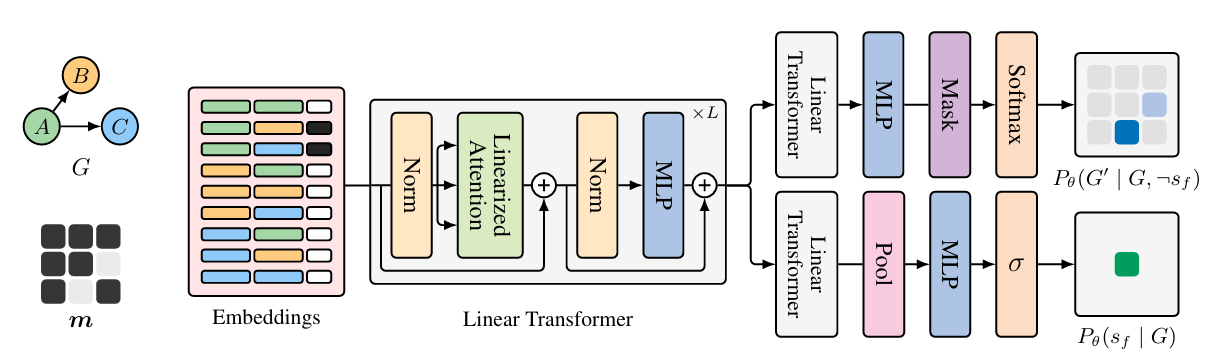
\includegraphics{figures/nn_architecture}
        \caption{Neural Network Architecture used in the proposed approach. Figure taken from~\cite{deleu2022daggflownet}.
        The input Graph $G$ is embedded into an embedding of $d^2$ edges where each edge is itself embedded using
        embedding of its outgoing and incoming nodes along with an indicator of its presence in the graph. A linear Transformer
        with $L$ layers is used and the output is passed through two different heads to copmute the terminating and non-terminating
        forward transition probabilities. Note that for $P_{\phi}(G_{i+1} \mid G_i, \neg s_f)$, the output is passed through a
        masking later filtering out invalid actions before using a softmax layer to normalize the probabilities.}
        \label{fig:nn_architecture}
    \end{figure}

    \textbf{The loss function} Now that we have defined the overall architecture of the neural network and the
    transition probabilities, we need to define the loss function to train the network.
    To satisfy eq.~\eqref{eq:detailed_balance}, authors suggested using the following loss function:
    \begin{equation}
        \mathcal{L}(\phi) = \sum_{G_i \to G_{i+1}} \left \log
        \frac{R(G_{i+1})P_{\psi}(G_i \mid G_{i+1})P_{\phi}(s_f \mid G_i)}{R(G_i)P_{\phi}(G_{i+1} \mid G_i)P_{\phi}(s_f \mid G_{i+1})} \right^2 .
        \label{eq:loss_function}
    \end{equation}

    Note that this loss function is only a function of $\phi$ and not $\psi$. This is because the backward transition
    is considered to be fixed and not learned.




    \bibliographystyle{ieee_fullname}
    \bibliography{references}

    \makeappendix

    \appendix

%\begin{thebibliography}{99}
%\end{thebibliography}

\end{document}
